\section{Data Description}\label{sec:data_description}
The primary data employed are located menu expenditures, which contain the yearly allotted allocations from Aldermen and their respective locations from 2005 to 2022.
This dataset comes from Menu spending reports that are publicly available from 2011 through 2022, and records that were not previously publicly available that were obtained through a FOIA request to Chicago's office of budget and management \cite{OBM_datasource}.  
I then scraped these PDFs and used the resulting cost total, ward, and location description data to create map of shapes of the locations of the expenditures.
I then used the location description text to to locate the described vertices of each project using the Census' geocoding API. 
If the census's API failed, google maps' API would be used instead.
In total, there were 43,596 projects that needed to be located, and 83\% of them were successfully located using one of the two above methods.
For example, spending on playground equipment would be a singular point, while spending on a street would be a line, and spending of all alleys within a given block would be a polygon.
This dataset contain 41,381 precinct-year observations which record the total amount of spending in a given voting precinct in a given year.
The variable of analysis is the annual fraction of observed spending on a given precinct in its ward in a given year.
``Observed'' here means that it was successfully located using the above methods.
Thus, if $Y_{py}$ is the fraction of spending located in precinct $p$ in year $y$, then $Y_{py} = \frac{S_{py}}{S_{wy}}$, where $S_{py}$ is the spending in precinct $p$ in year $y$, and $S_{wy}$ is the total amount of ward $w$'s spending that was successfully located in year $y$.

Below in table~\ref{summary_stats} 

Below in Figure~\ref{fig:spending_hist} are two side-by-side histograms of the distribution of spending per precinct aggregated across the 2005-2011 period which used the 2003-2011 ward boundaries, and the 2012-2022 period with the 2012-2022 ward boundaries.
We generally see that the decentralized nature of the menu program leads to a large variation in spending per precinct, but the distribution has a long right tail.
Both figures are winsorized at the 99th percentile to remove outliers.

\begin{figure}[H]
    \centering
    % First subfigure
    \begin{subfigure}[b]{0.45\textwidth} % [b] aligns at the bottom
      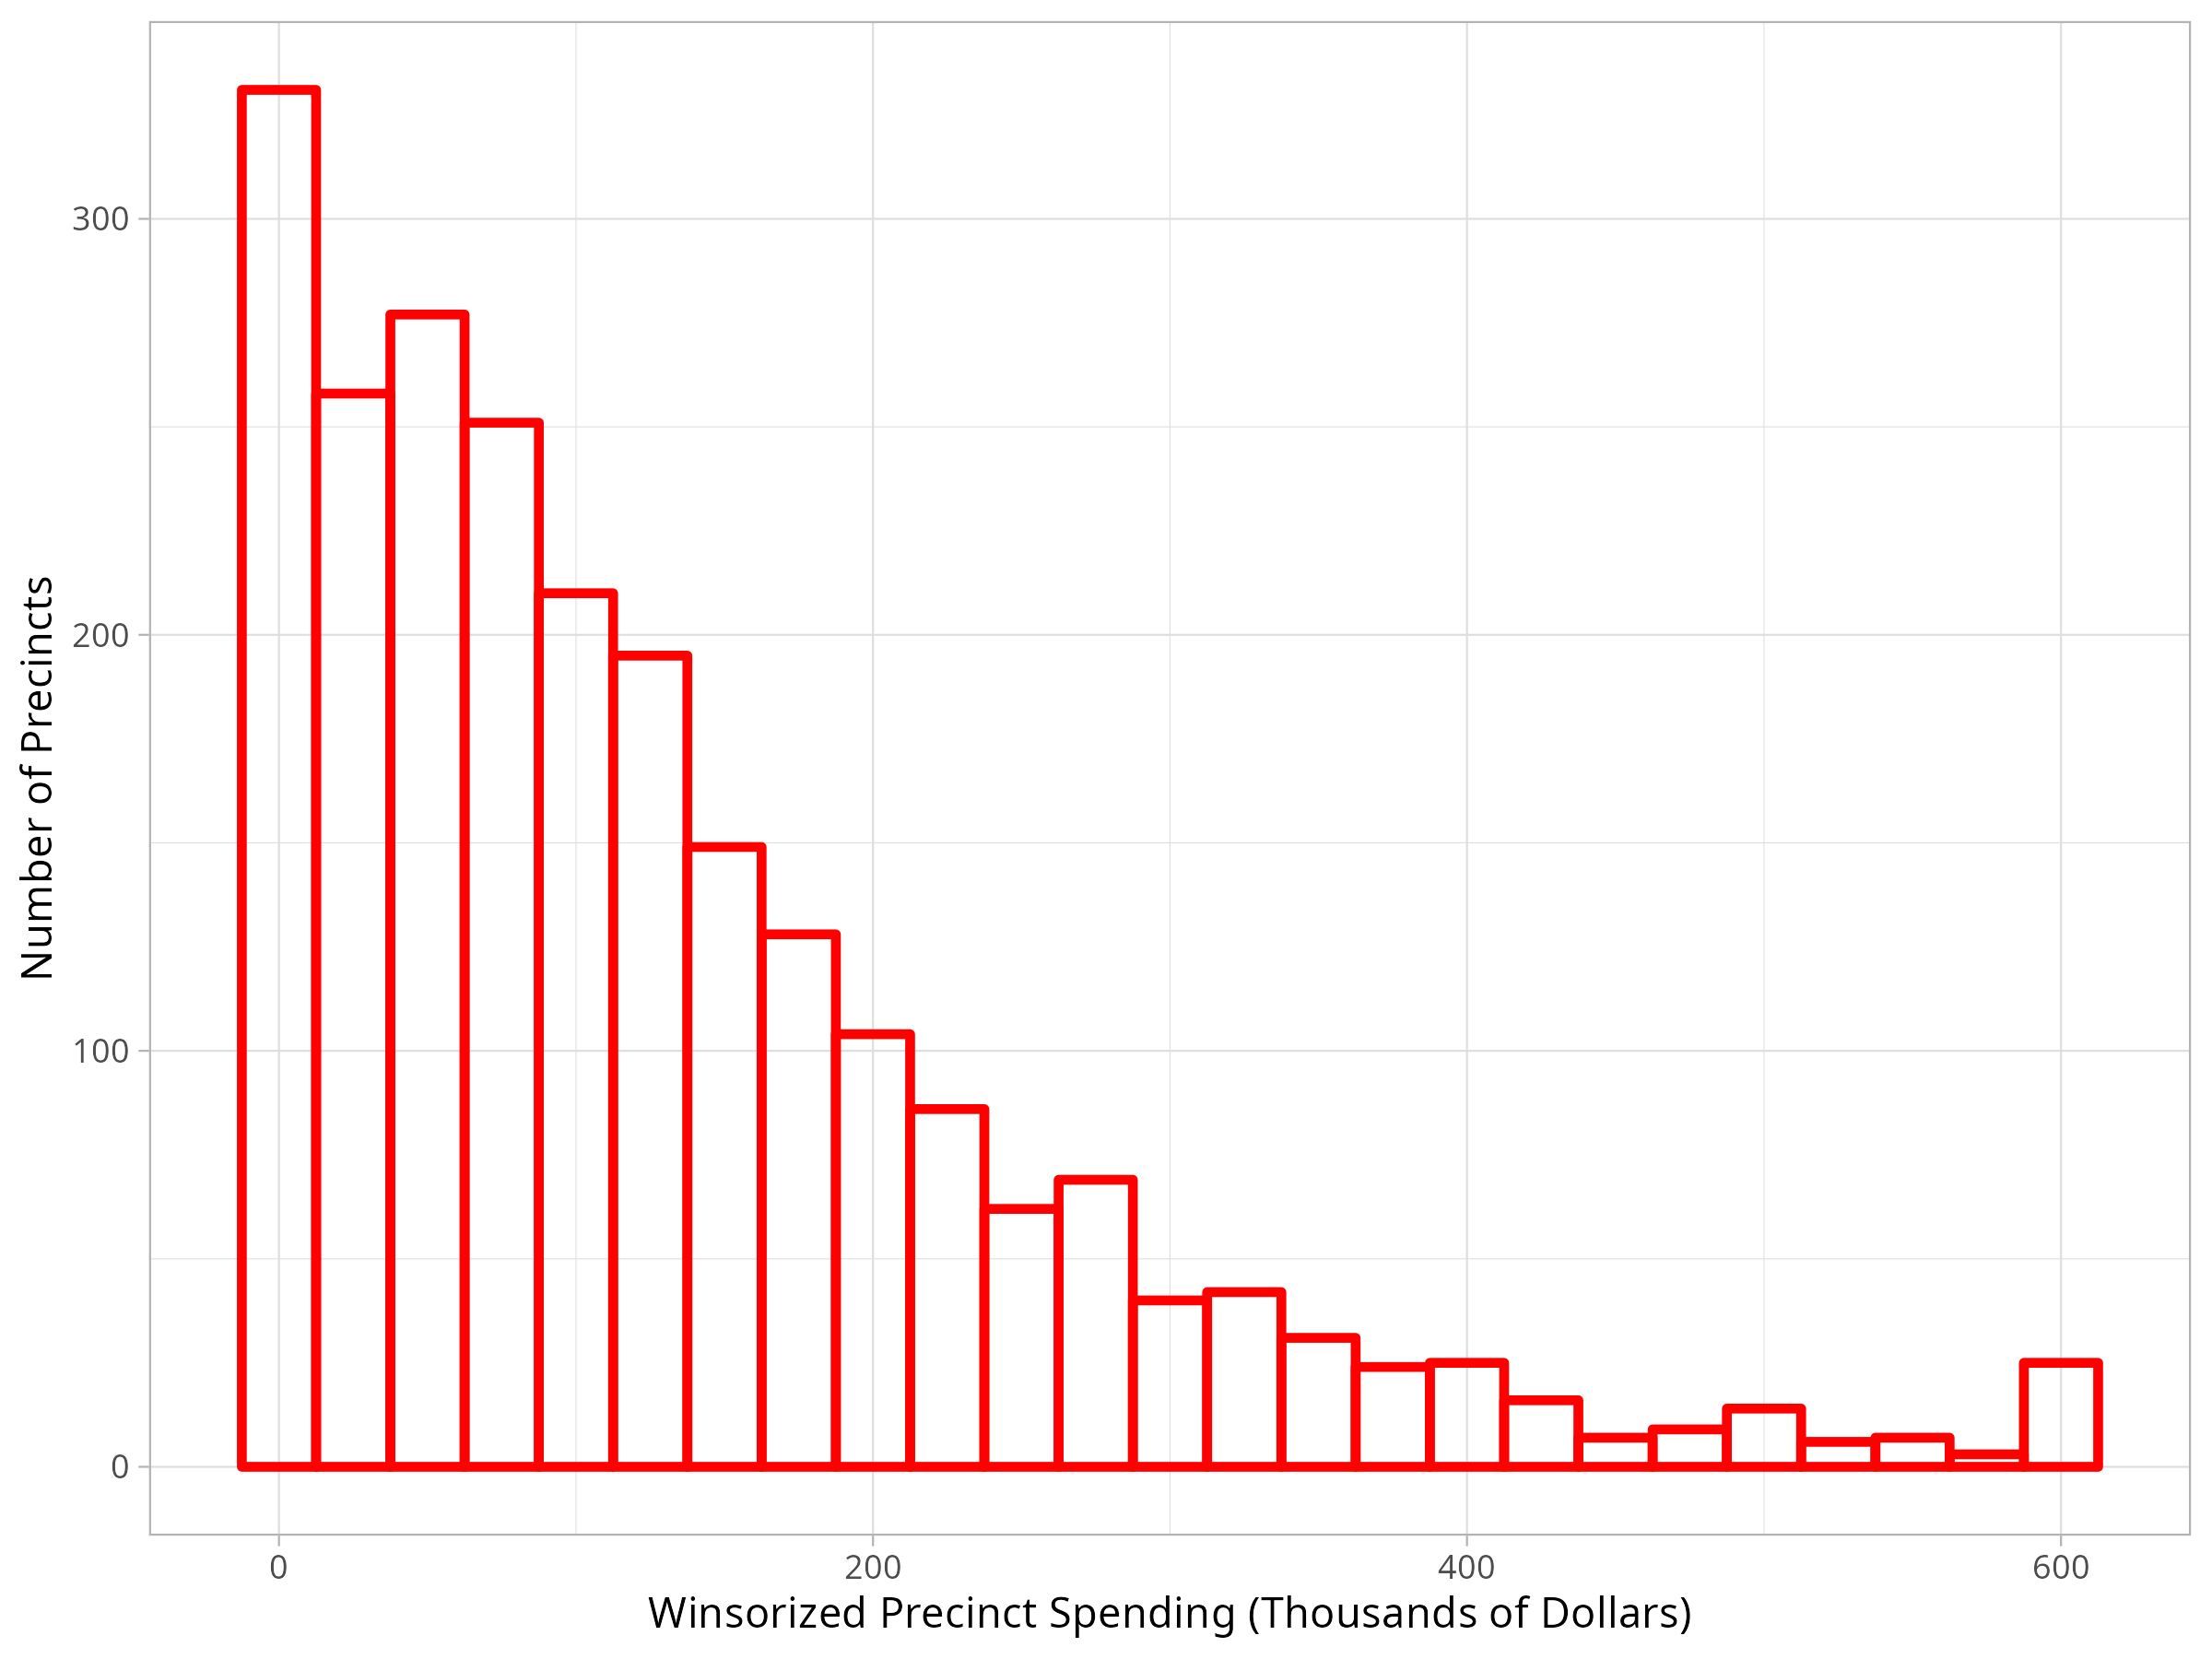
\includegraphics[width=\textwidth]{input/spending_histogram_2005_2011.png}
      \caption{Distribution of Spending per Precinct, 2005-2011}
      \label{fig:sub1}
    \end{subfigure}
    \hfill % This adds some space between the two subfigures
    % Second subfigure
    \begin{subfigure}[b]{0.45\textwidth}
      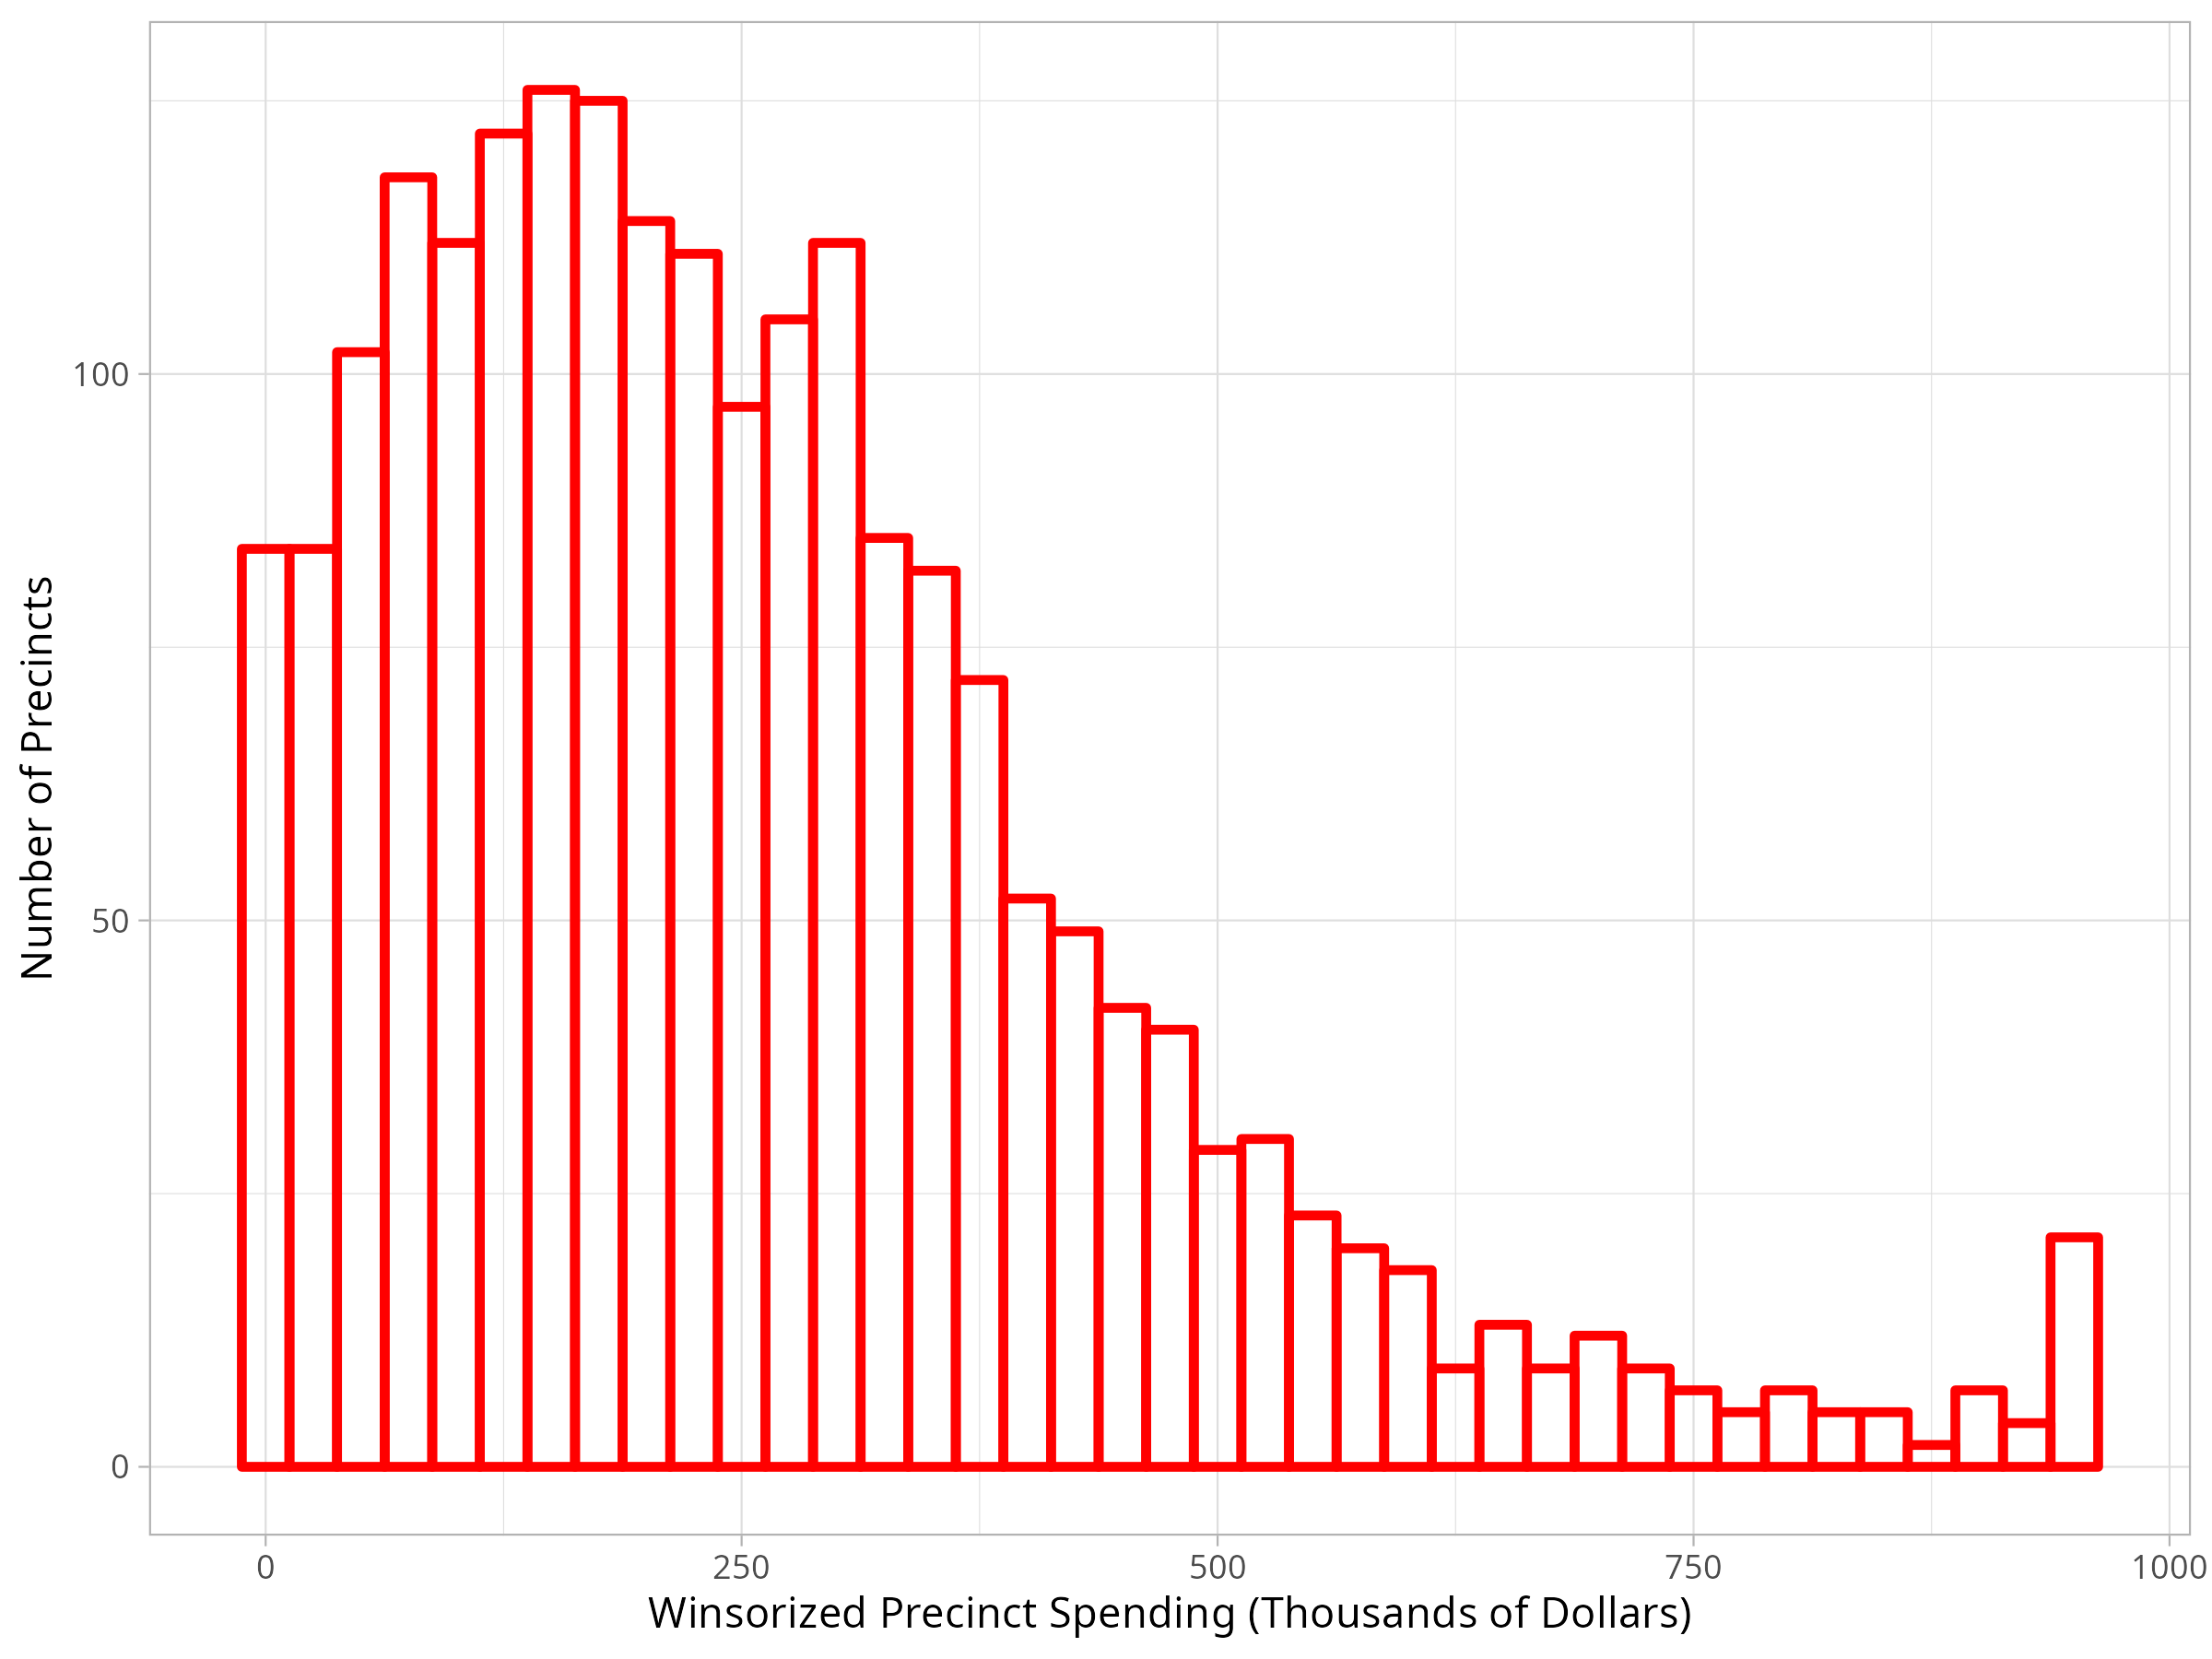
\includegraphics[width=\textwidth]{input/spending_histogram_2012_2022.png}
      \caption{Distribution of Spending per Precinct, 2012-2022}
      \label{fig:sub2}
    \end{subfigure}
  
    \caption{Distribution of Spending per Precinct for both ward maps in the dataset}
    \label{fig:spending_hist}
  \end{figure}

Next we can visualize how the decentralized nature of the menu program leads to large within-precinct spending variation through a map of the 2012-2022 spending per precinct in Figure~\ref{fig:spending_map}.
This figures shows how the program's decentralization leads to numerous precincts with large concentrations of spending.
Furthermore, the figure shows that in some wards, spending is heavily concentrated in a few precincts, while in others, spending is more evenly distributed.

\begin{figure}[H]
    \centering
    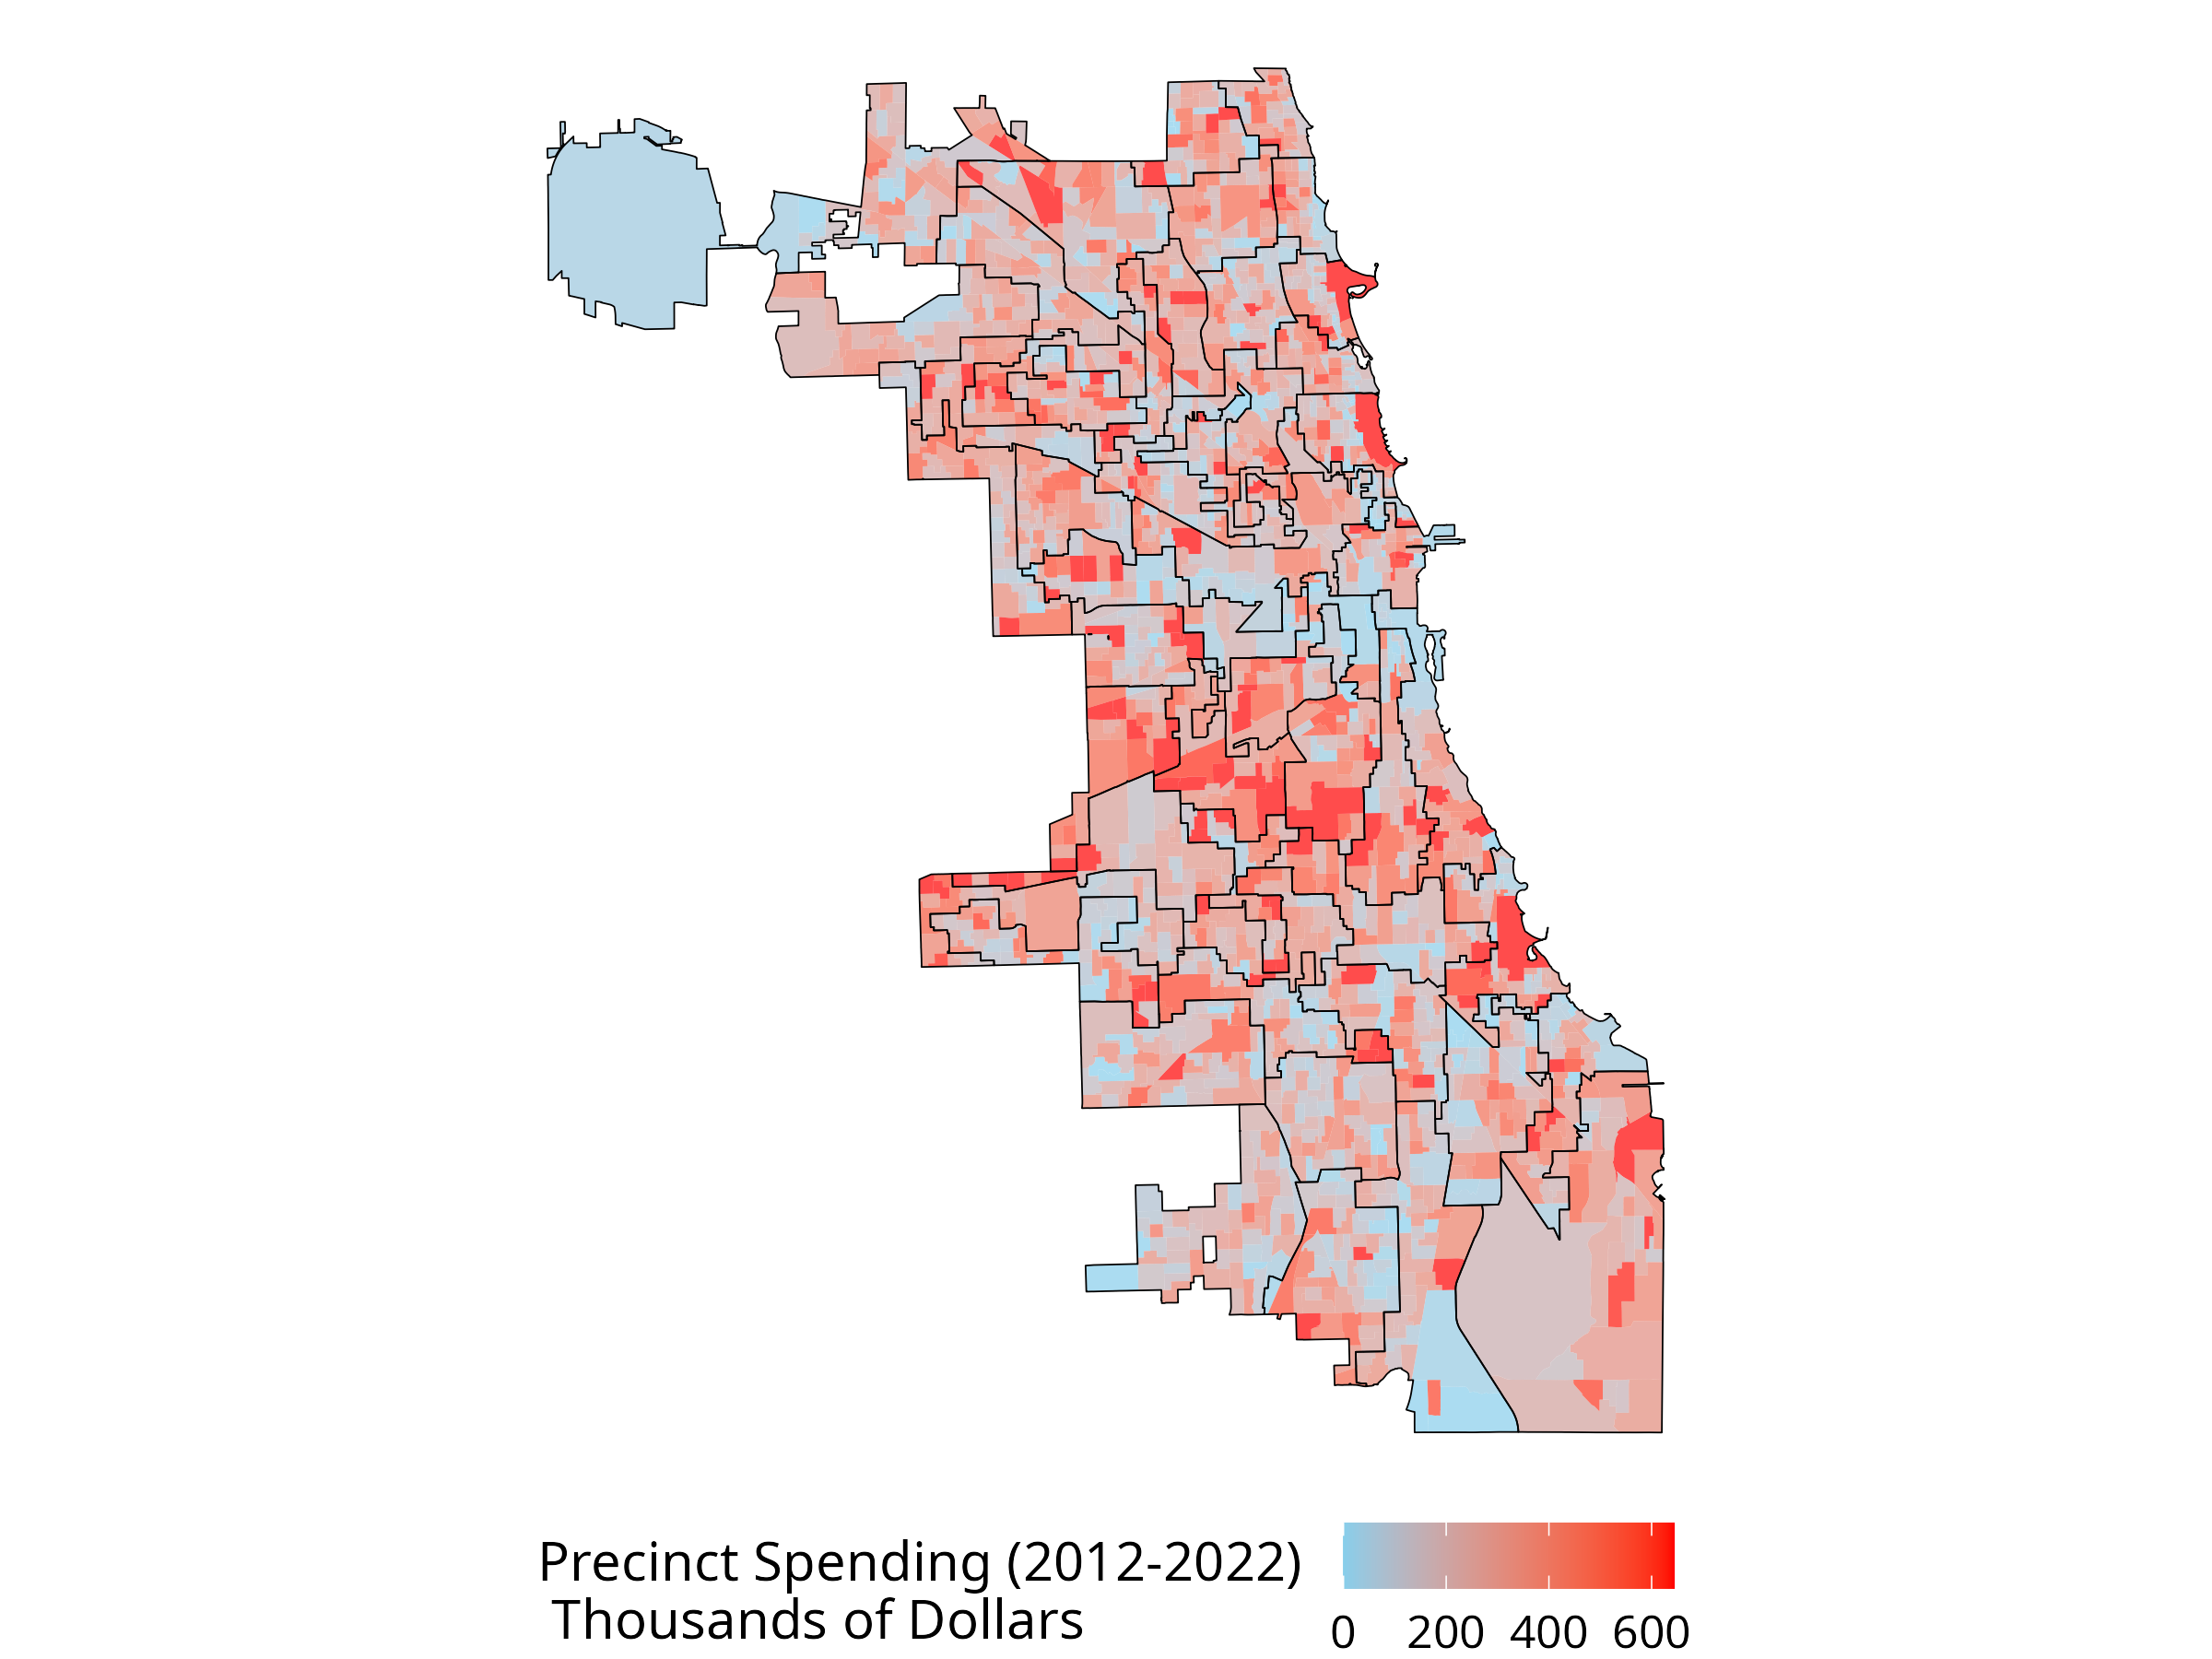
\includegraphics[width=0.8\textwidth]{input/whole_chicago_map_2012_2022.png}
    \caption{Map of Spending per Precinct, 2012-2022}
    \label{fig:spending_map}
\end{figure}

\textcolor{red}{\textbf{TODO:} Add a scatterplot of spending fraction per precinct vs. net votes for the incumbent alderman}